\documentclass[11pt,a4paper]{article}
\usepackage[spanish,provide=*]{babel}
\usepackage{fontspec}
\usepackage[margin=2.4cm]{geometry}
\usepackage{graphicx,booktabs,tabularx,float,microtype,enumitem,xcolor}
\usepackage[font=small,labelfont=bf]{caption}
\usepackage{xurl}
\usepackage[colorlinks=true,linkcolor=black,citecolor=black,urlcolor=blue!50!black]{hyperref}
\captionsetup[table]{name=Tabla}
\captionsetup[figure]{name=Figura}
\setlength{\parskip}{4pt}
\setlength{\parindent}{0pt}
\setlist{nosep,leftmargin=1.2em}
\graphicspath{{../resultados/}}
\newcommand{\cita}[1]{[#1]}
\makeatletter\let\inputtab\@@input\makeatother

\begin{document}

% ---------------------------------------------------------------- PORTADA
\begin{titlepage}
\centering
\vspace*{2cm}
{\large Universidad Externado de Colombia\\Facultad de Ciencia de Datos\par}
\vspace{0.6cm}
{\large Machine Learning I · Proyecto Integrador · Fase 3 (entrega final)\par}
\vspace{2.5cm}
{\LARGE\bfseries Predicción del bajo peso al nacer en Colombia\\[0.3em] con datos reales del DANE (nacimientos 2022)\par}
\vspace{0.8cm}
{\large Modelo final, interpretación y contraste con Feyisa \emph{et al.} (2023)\par}
\vspace{2.5cm}
{\large Daniel Felipe Galeano Peña\par}
\vspace{0.3cm}
{Docente: Diana Pulido\par}
\vfill
{Código y datos: \url{https://github.com/Galeo2906/proyecto-ml-bajo-peso-nacer}\par}
\vspace{0.3cm}
{Bogotá, noviembre de 2026\par}
\end{titlepage}

% ---------------------------------------------------------------- 1
\section{Problema, datos y qué se corrigió}

El bajo peso al nacer (BPN, menos de 2.500 g) aumenta el riesgo de muerte neonatal y de problemas de desarrollo. El artículo base \cita{1}, un estudio de casos y controles con 324 madres del oeste de Etiopía, encontró cuatro factores asociados: no recibir consejería nutricional (OR 2,4), perímetro braquial menor de 23 cm (OR 3,1), estrés durante el embarazo (OR 2,8) y menos de cuatro controles prenatales (OR 2,8). La pregunta de este proyecto es doble: \textbf{(i)} ¿qué tan bien se puede anticipar el BPN en Colombia con la información que se registra antes del parto? y \textbf{(ii)} ¿se reproducen en el contexto colombiano los hallazgos del artículo?

\textbf{Datos reales.} Se usaron los microdatos de Estadísticas Vitales del DANE, nacimientos 2022 \cita{2}: 573.625 registros, de los cuales 567.766 tienen el peso informado y el 10,48~\% tiene BPN. Se trabajó con una muestra aleatoria simple de 50.000 nacimientos (semilla 42); tras excluir los 477 sin peso quedan 49.523, con 10,42~\% de BPN, es decir, la muestra es representativa. Los códigos de cada variable se tomaron del certificado de nacido vivo y de las agrupaciones publicadas por el DANE \cita{3,4}. Solo entran variables conocidas \emph{antes} del parto: edad, educación, estado conyugal, etnia, régimen de salud, zona y región de residencia de la madre, embarazo múltiple, número de hijos, pérdidas previas y número de controles prenatales. Se excluyeron, por fuga, las semanas de gestación, la talla, el Apgar, el tipo de parto, quién lo atendió y el sexo del recién nacido.

\textbf{Variable objetivo y codificación.} El DANE no publica el peso exacto, sino rangos codificados en \texttt{PESO\_NAC} (1: menos de 1.000 g; 2: 1.000--1.499; 3: 1.500--1.999; 4: 2.000--2.499; 5 a 8: 2.500 g o más; 9: sin información). La variable objetivo se obtiene al \emph{dicotomizar} esa columna: vale 1 para los códigos 1 a 4 (menos de 2.500 g) y 0 para los códigos 5 a 8; los registros con código 9 se excluyen. Esta variable es la respuesta que el modelo aprende a predecir y nunca entra como predictora. Las 11 variables predictoras son categóricas, así que el \texttt{Pipeline} las convierte en variables indicadoras (\emph{dummies} o one-hot): una columna 0/1 por categoría, 54 en total. En la regresión logística cada indicadora se compara con una categoría de referencia, la más frecuente de cada variable (por ejemplo, región Andina o 7 o más controles); por eso cada odds ratio se lee como ``frente a'' esa referencia.

\textbf{Qué muestran los datos antes de modelar.} Sin ajustar por nada, las diferencias grandes se concentran en pocas variables: el 69,6~\% de los embarazos múltiples termina en BPN, frente al 9,3~\% de los simples; el 15,0~\% de las madres con menos de cuatro controles tiene un bebé con BPN, frente al 7,6~\% de las que tuvieron siete o más; Bogotá llega a 15,3~\%, mientras Orinoquía-Amazonía queda en 7,2~\%; y las edades extremas tienen más riesgo (17,1~\% entre los 10 y 14 años y 13,7~\% entre los 40 y 44). Educación, zona y régimen de salud apenas mueven la tasa (entre 8~\% y 11~\%). Esto ya anticipa que el modelo tendrá pocas señales fuertes y muchas débiles.

\textbf{Correcciones de la segunda entrega} (Tabla~\ref{tab:correcciones}). La simulación se retiró y todo el análisis usa datos reales; la comparación usa solo modelos vistos en clase; se corrigió el error por el que la L1 y el Elastic Net eran en realidad una L2 (ahora se fija \texttt{penalty} y se verifica, Sección~\ref{sec:modelo}); y todas las tablas y figuras de este informe salen del cuaderno entregado.

\begin{table}[H]
\centering\small
\caption{Observaciones de la retroalimentación de la segunda entrega y cómo se atendieron.}
\label{tab:correcciones}
\begin{tabularx}{\textwidth}{>{\raggedright\arraybackslash}p{5.4cm}X}
\toprule
Observación & Qué se hizo \\
\midrule
Sin datos reales locales & Microdatos reales del DANE 2022; la simulación se retira. \\
Modelos no vistos en clase como eje de la decisión & Solo modelos del curso; el modelo final es la logística sin penalizar. La regularización, LDA y QDA quedan como comparación declarada y sustentada (Sección~\ref{sec:modelo}). \\
L1 y Elastic Net no fijaban \texttt{penalty} & \texttt{penalty="l1"}/\texttt{"elasticnet"} con \texttt{solver="saga"}, verificado: con $C=0{,}01$ la L1 deja 33 de 54 coeficientes en cero y la L2 ninguno. \\
Tablas del informe distintas al cuaderno & Las tablas se generan desde los CSV del cuaderno (\texttt{generar\_tablas\_informe.py}). \\
Bibliografía incompleta; 9 páginas & Referencias completas; cuerpo dentro del límite. \\
\bottomrule
\end{tabularx}
\end{table}

\textbf{Flujo sin fuga.} Partición 80/20 estratificada (39.618 para entrenar, 9.905 para la prueba, que se usa una sola vez). Cada modelo es un único \texttt{Pipeline} de scikit-learn \cita{9}: codificación one-hot aprendida solo del entrenamiento, escalamiento cuando el modelo lo necesita y el clasificador. La comparación usa validación cruzada anidada: 5 pliegues $\times$ 2 repeticiones por fuera (10 estimaciones, para medir estabilidad) y búsqueda de hiperparámetros con 3 pliegues por dentro. La métrica principal es la PR-AUC, porque con 10~\% de casos la exactitud engaña (decir ``nadie tiene BPN'' acierta el 90~\%) y la PR-AUC se concentra en la clase que importa \cita{5}; su valor de azar es la prevalencia (0,104). Como complemento se reportan la ROC-AUC (capacidad de ordenar, con azar en 0,5), el Brier (error cuadrático de las probabilidades: mide si un ``20~\% de riesgo'' significa de verdad 20~\%) y, una vez fijado un umbral, el recall (qué parte de los casos se detecta) y la precisión (qué parte de las alarmas es un caso real). Las decisiones de preprocesamiento dependen del modelo: KNN y Naive Bayes trabajan sobre las columnas 0/1 sin escalar (escalar haría pesar más las categorías raras en la distancia), y para Naive Bayes se usa la versión Bernoulli, que es la que corresponde a variables binarias; las logísticas y QDA se escalan para que la penalización sea justa entre variables.

% ---------------------------------------------------------------- 2
\section{Modelo final}\label{sec:modelo}

Se compararon nueve modelos del curso (Tabla~\ref{tab:cv}, Figura~\ref{fig:cv}). \textbf{Las cuatro logísticas y LDA empatan} (PR-AUC 0,273--0,274, unas 2,6 veces el azar) y son estables (desviación de 0,012 entre pliegues); la mayor diferencia entre ellas (0,0003) es unas 40 veces menor que esa variación, así que no son distinguibles. Naive Bayes queda algo por debajo y es más variable; QDA y KNN son claramente peores, y QDA además está peor calibrado que la línea base (Brier 0,113 frente a 0,093).

\begin{table}[H]
\centering\small
\caption{Comparación en validación cruzada anidada (entrenamiento, 10 pliegues externos). Media $\pm$ desviación estándar. El hiperparámetro es el más elegido por la búsqueda interna.}
\label{tab:cv}
\begin{tabular}{lcccc}
\toprule
Modelo & PR-AUC & ROC-AUC & Brier & Hiperparámetro \\
\midrule
\inputtab{tablas/tab_cv.tex}
\bottomrule
\end{tabular}
\end{table}

\begin{figure}[H]
\centering
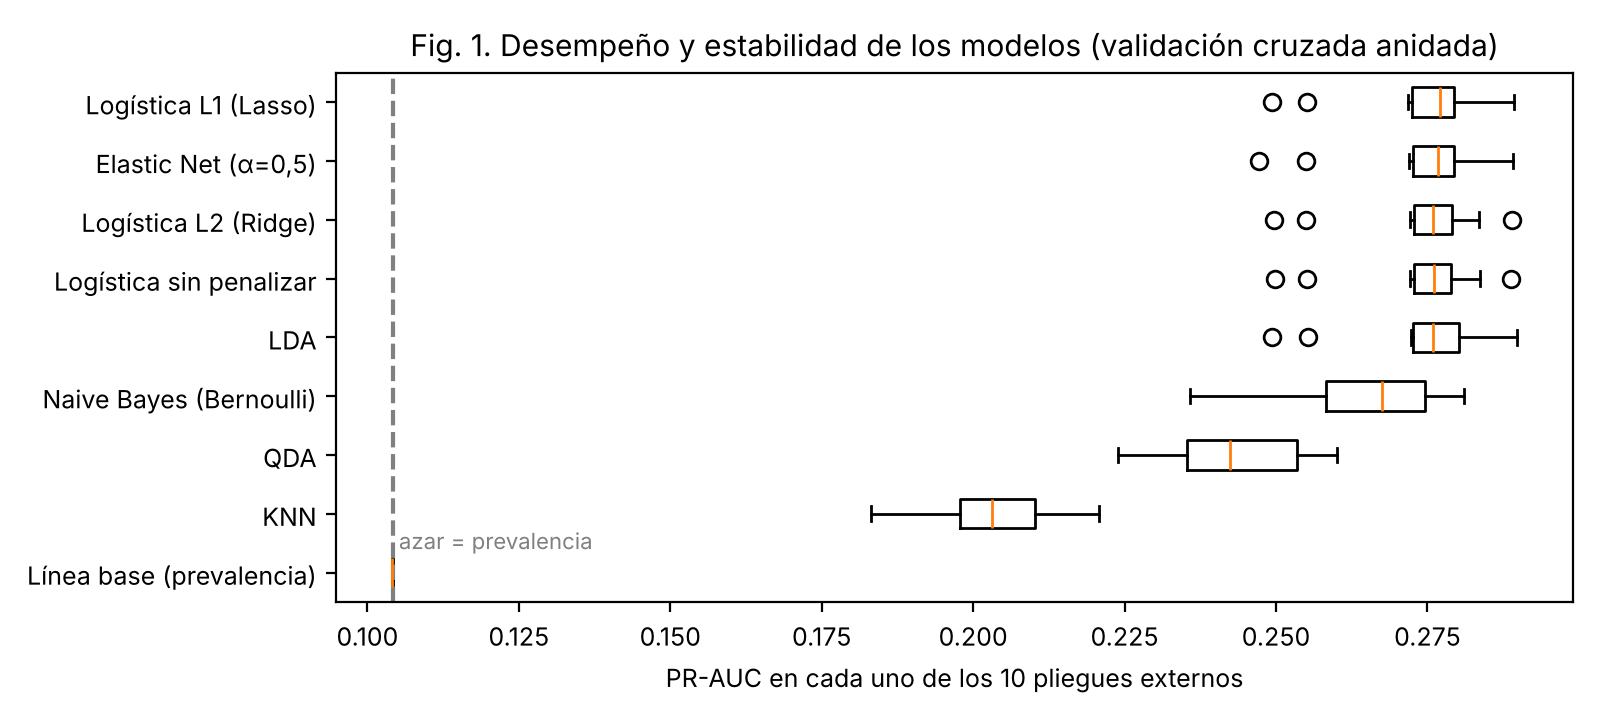
\includegraphics[width=0.82\textwidth]{fig1_estabilidad_cv.png}
\caption{PR-AUC de cada modelo en los 10 pliegues externos. \textbf{Qué leer:} las logísticas y LDA forman un bloque estable y superpuesto; KNN y QDA quedan claramente atrás, y todos superan el azar (línea punteada).}
\label{fig:cv}
\end{figure}

\textbf{Regla de selección (fijada antes de ver los resultados).} Entre los modelos a menos de una desviación estándar del mejor, se elige el más interpretable. La L1 tuvo la media más alta (0,2736 $\pm$ 0,0123), pero la logística sin penalizar (0,2733) está dentro del margen, entrega odds ratios directos ---el mismo método del artículo--- y comparte con las demás logísticas la mejor calibración (Brier 0,0851). \textbf{El modelo final es la regresión logística sin penalizar}, con umbral de decisión elegido por F2 sobre predicciones fuera de muestra del entrenamiento (0,082). F2 pesa el recall el doble que la precisión porque, en salud pública, no detectar un caso cuesta más que una alarma de más.

\textbf{Configuración definitiva.} Un \texttt{Pipeline} con \texttt{OneHotEncoder} (categorías nuevas ignoradas), \texttt{StandardScaler} y \texttt{LogisticRegression(penalty=None)}, con 11 variables categóricas que se convierten en 54 columnas; sin hiperparámetros que ajustar; umbral de decisión 0,082 (cuando el riesgo predicho supera 8,2~\%, la gestante se marca como de riesgo; es bajo porque el BPN es poco frecuente). Se entrenó una sola vez con todo el 80~\% y se evaluó una sola vez en el 20~\% reservado. Semilla 42 en la muestra, la partición, la validación cruzada y el bootstrap; el cuaderno corre de principio a fin en unos 25 minutos.

\textbf{¿Por qué no la regularización?} La penalización L2 encoge los coeficientes y la L1 además apaga algunos, para reducir la varianza cuando hay pocos datos por parámetro (Sesiones 37--38; \cita{8}). Aquí hay unos 40.000 registros para 54 coeficientes: la varianza ya es pequeña. La Figura~\ref{fig:curvas} lo muestra: con $C \geq 0{,}01$ las tres penalizaciones rinden igual que el modelo sin penalizar, y solo con $C=0{,}001$ (castigo muy fuerte) se pierde desempeño porque la L1 apaga 52 de los 54 coeficientes. La búsqueda eligió $C=0{,}1$, en plena meseta. Regularizar no mejora nada y haría perder la lectura directa de los odds ratios. En KNN el desempeño sube con $k$ (el mejor fue 401, el borde de la rejilla): con variables categóricas hay muchos registros idénticos y KNN termina promediando grupos grandes; aun así queda lejos.

\begin{figure}[H]
\centering
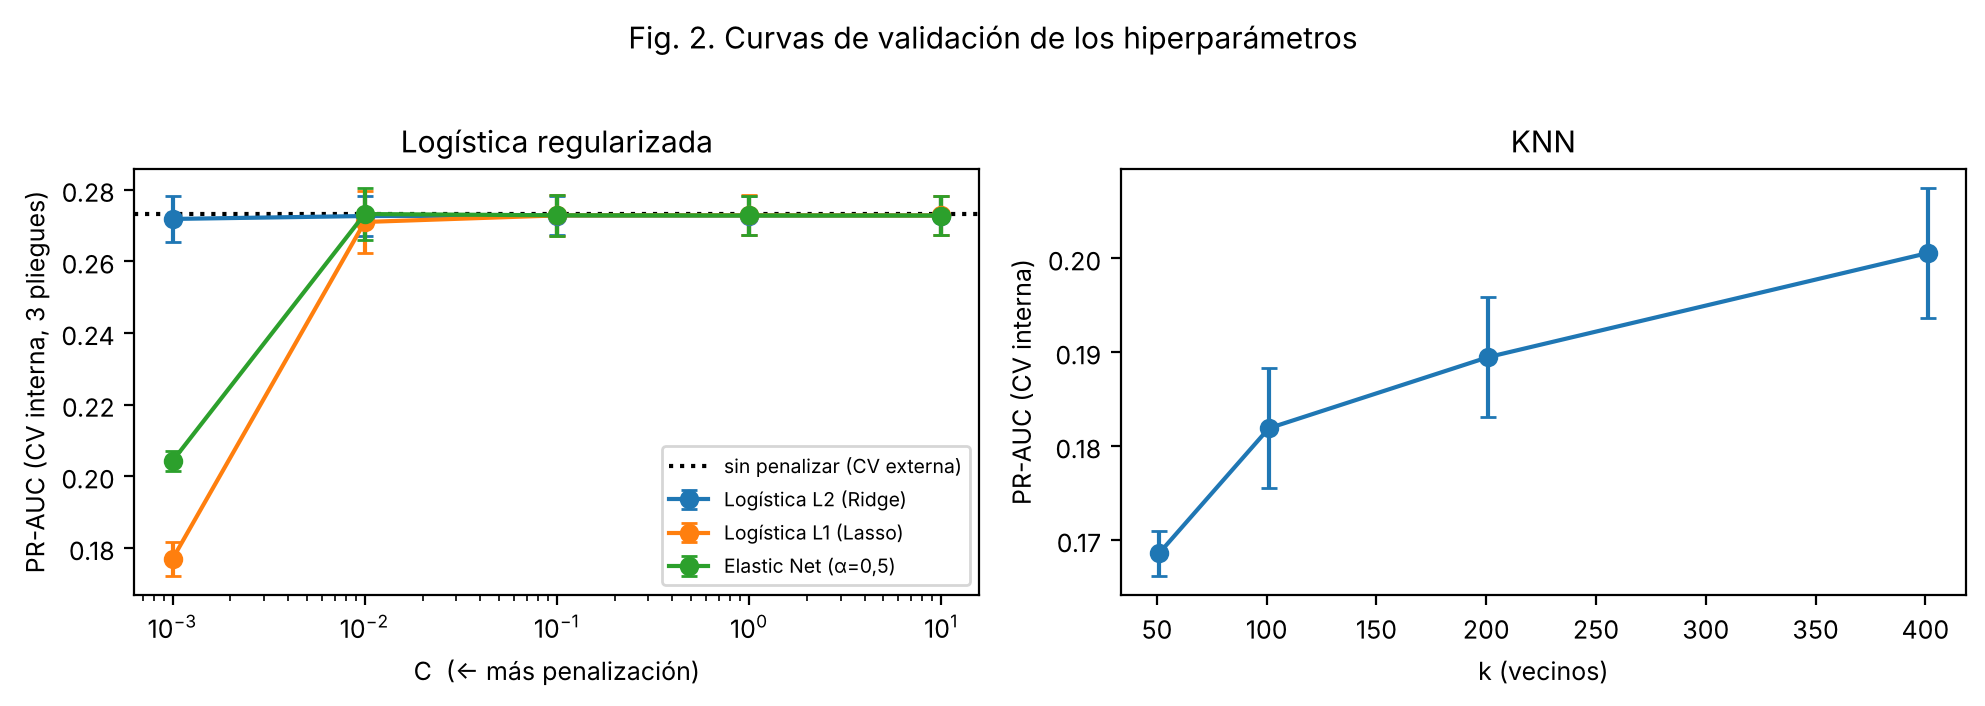
\includegraphics[width=0.95\textwidth]{fig2_curvas_validacion.png}
\caption{Curvas de validación. \textbf{Qué leer:} la regularización solo cambia el resultado cuando es extrema ($C=0{,}001$); en el resto coincide con la logística sin penalizar (línea punteada).}
\label{fig:curvas}
\end{figure}

\textbf{Supuestos de LDA y QDA.} Ambos suponen normalidad multivariada dentro de cada clase, que no se cumple con variables 0/1. LDA supone además covarianzas iguales: la razón de varianzas entre clases tiene mediana 1,01, así que el supuesto es razonable salvo en embarazo múltiple (varianza unas 18 veces mayor entre los casos). Por eso LDA discrimina igual que la logística (ambas llegan a una frontera lineal parecida) pero calibra peor (Brier 0,0872). QDA estima una covarianza por clase con solo unos 4.100 casos de BPN y 54 columnas binarias; sin regularizarla no se puede estimar, y aun con \texttt{reg\_param} = 0,5 es el peor calibrado.

% ---------------------------------------------------------------- 3
\section{Interpretación de resultados}

\textbf{Desempeño en la prueba (usada una sola vez).} La PR-AUC es 0,266 (IC 95~\%: 0,240--0,292), muy cercana a la de validación cruzada (0,273): no hay sobreajuste (Tabla~\ref{tab:prueba}). La ROC-AUC de 0,663 significa que, si se toma al azar un bebé con BPN y uno sin BPN, el modelo le asigna más riesgo al primero dos de cada tres veces. Es un modelo \textbf{modesto}: ordena el riesgo mejor que el azar, pero no diagnostica.

\begin{table}[H]
\centering\small
\caption{Evaluación única del modelo final (logística sin penalizar) en el 20~\% de prueba. IC por bootstrap (1.000 remuestreos).}
\label{tab:prueba}
\begin{tabular}{lcc}
\toprule
Métrica & Valor & Referencia \\
\midrule
\inputtab{tablas/tab_prueba.tex}
\bottomrule
\end{tabular}
\end{table}

\textbf{Los errores y su costo.} Con el umbral F2, por cada 1.000 nacimientos el modelo detecta 73 casos de BPN, deja pasar 31, da 444 falsas alarmas y descarta correctamente a 452 (Figura~\ref{fig:prueba}a). Los dos errores no cuestan lo mismo: un falso negativo es un bebé de bajo peso cuya madre no recibió vigilancia adicional; un falso positivo es, por ejemplo, una ecografía de crecimiento de más. Aun así, marcar a la mitad de las gestantes no es práctico. El uso más realista es \textbf{priorizar}: el quintil de mayor riesgo tiene 20,3~\% de BPN, el doble del promedio, y concentra el 39~\% de los casos con solo el 20~\% de los nacimientos (Figura~\ref{fig:prueba}c). Las probabilidades están bien calibradas (Figura~\ref{fig:prueba}b): cuando el modelo dice 15~\%, ocurre cerca del 15~\%.

\begin{figure}[H]
\centering
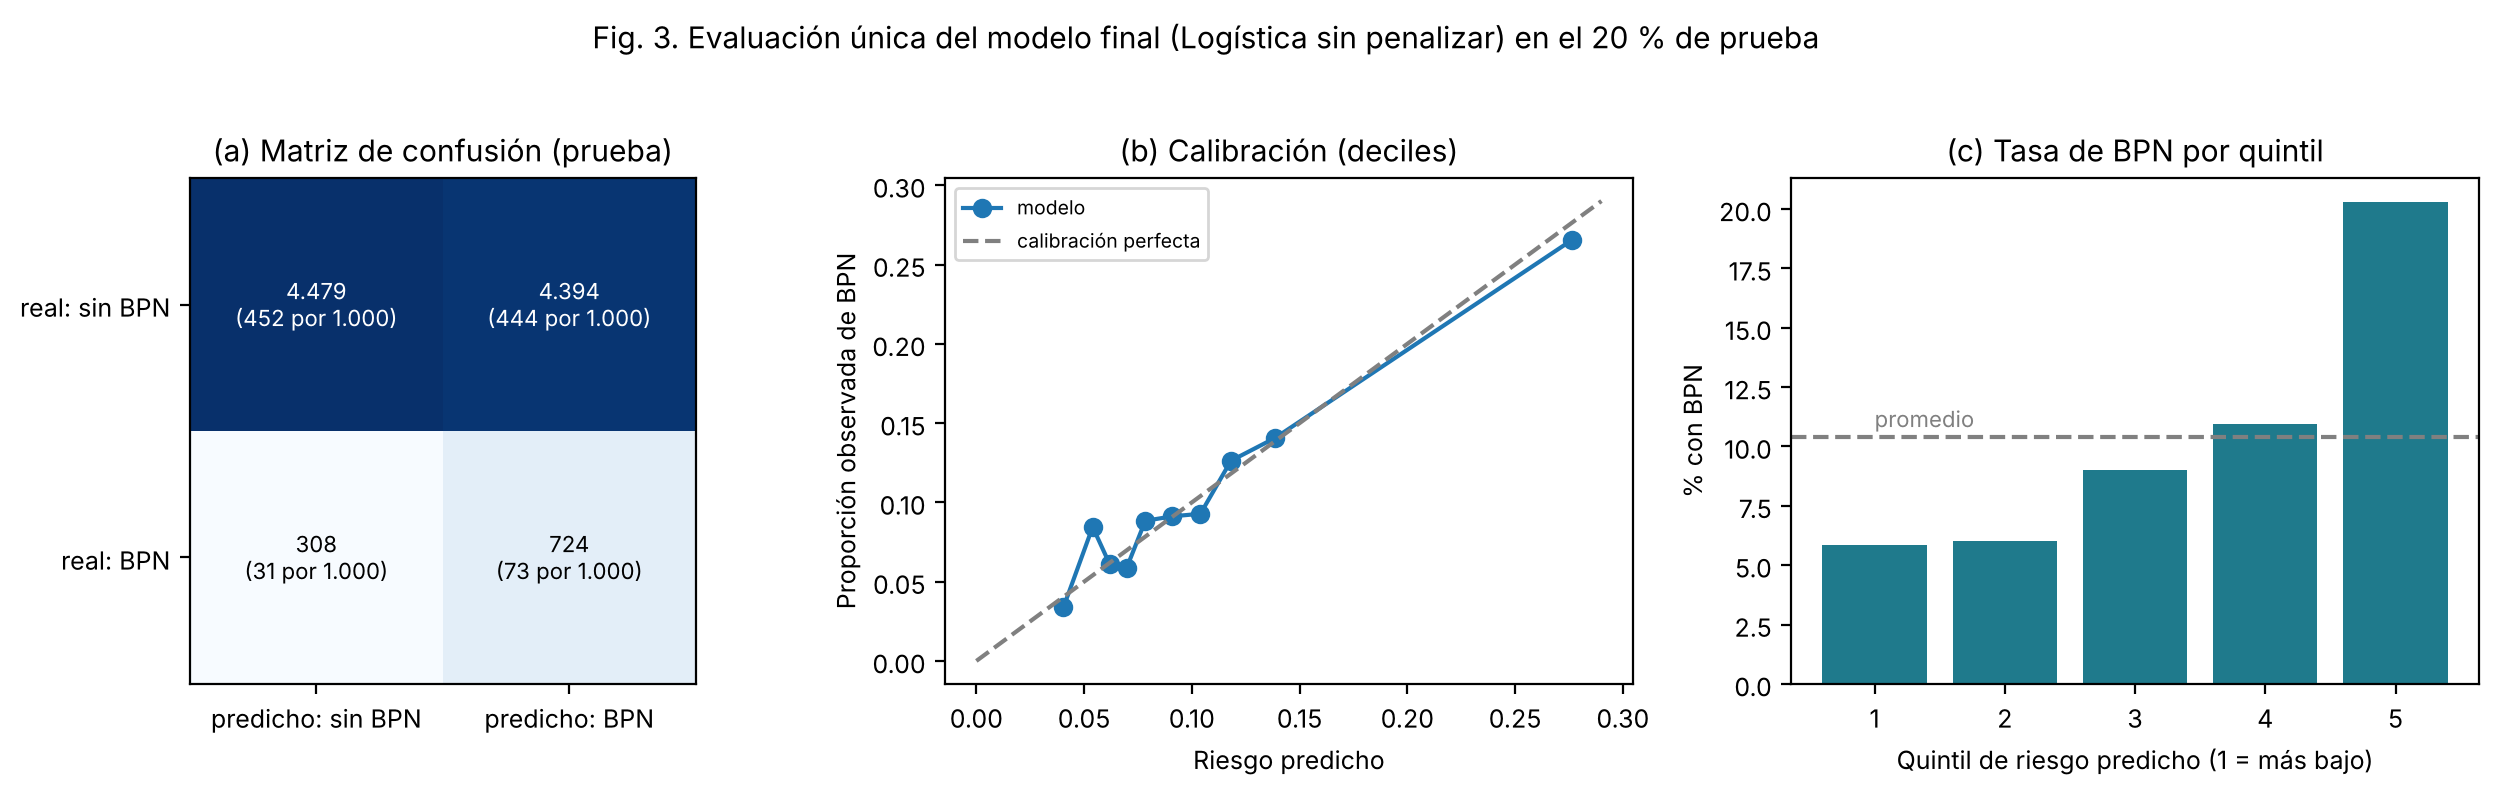
\includegraphics[width=\textwidth]{fig3_prueba_final.png}
\caption{Evaluación en prueba. \textbf{Qué leer:} (a) el modelo detecta 7 de cada 10 casos a cambio de muchas falsas alarmas; (b) las probabilidades coinciden con lo observado; (c) el riesgo se concentra en el quintil superior.}
\label{fig:prueba}
\end{figure}

\textbf{¿A quién no detecta?} De los 308 casos no detectados, ninguno es embarazo múltiple, solo el 2,3~\% tuvo menos de cuatro controles y el 77~\% tuvo siete o más. El modelo encuentra el BPN que deja huella en el certificado y no ve el que ocurre en embarazos aparentemente bien controlados, cuyas causas (preeclampsia, insuficiencia placentaria, desnutrición o estrés materno) no se registran en las estadísticas vitales. El límite lo pone la información disponible, no el algoritmo.

\textbf{¿Qué umbral usar en la práctica?} Depende de la capacidad del servicio de salud. Con el umbral F2 se detecta el 70~\% de los casos, pero hay que hacer seguimiento a la mitad de las gestantes (precisión de 14~\%). Si solo se puede reforzar el seguimiento del 20~\% de mayor riesgo, se detecta el 39~\% de los casos con una precisión del 20~\%, el doble que sin modelo. El modelo no decide por el médico; ofrece una forma ordenada de repartir un recurso escaso.

\textbf{Qué dice el modelo sobre el fenómeno} (Tabla~\ref{tab:or}, Figura~\ref{fig:or}). El embarazo múltiple multiplica las odds de BPN por unas 30. Los controles prenatales muestran un gradiente: menos de cuatro triplican las odds y de cuatro a seis casi las duplican, frente a siete o más. Residir en Bogotá aumenta las odds 1,5 veces aun ajustando por todo lo demás, lo que es coherente con el efecto de la altitud (2.600 m) sobre el crecimiento fetal \cita{6,7}. El riesgo es mayor en las edades extremas de la madre, en el primer hijo y cuando hubo pérdidas previas. Educación, zona, régimen y etnia tienen efectos pequeños una vez se ajusta por lo anterior. Dos resultados (madre no asegurada, OR 0,74; Orinoquía-Amazonía, OR 0,57) no deben leerse como protección: pueden reflejar quién queda registrado y la calidad del registro del peso en zonas apartadas.

\begin{table}[H]
\centering\small
\caption{Odds ratios ajustados de la logística, estimados con statsmodels \cita{10} (entrenamiento, $p<0{,}05$) y contraste con el artículo base. ``--'': el artículo no estudió esa variable.}
\label{tab:or}
\begin{tabular}{lcccc}
\toprule
Factor (vs. referencia) & OR & IC 95~\% & $p$ & OR Feyisa \emph{et al.} \\
\midrule
\inputtab{tablas/tab_or.tex}
\bottomrule
\end{tabular}
\end{table}

\begin{figure}[H]
\centering
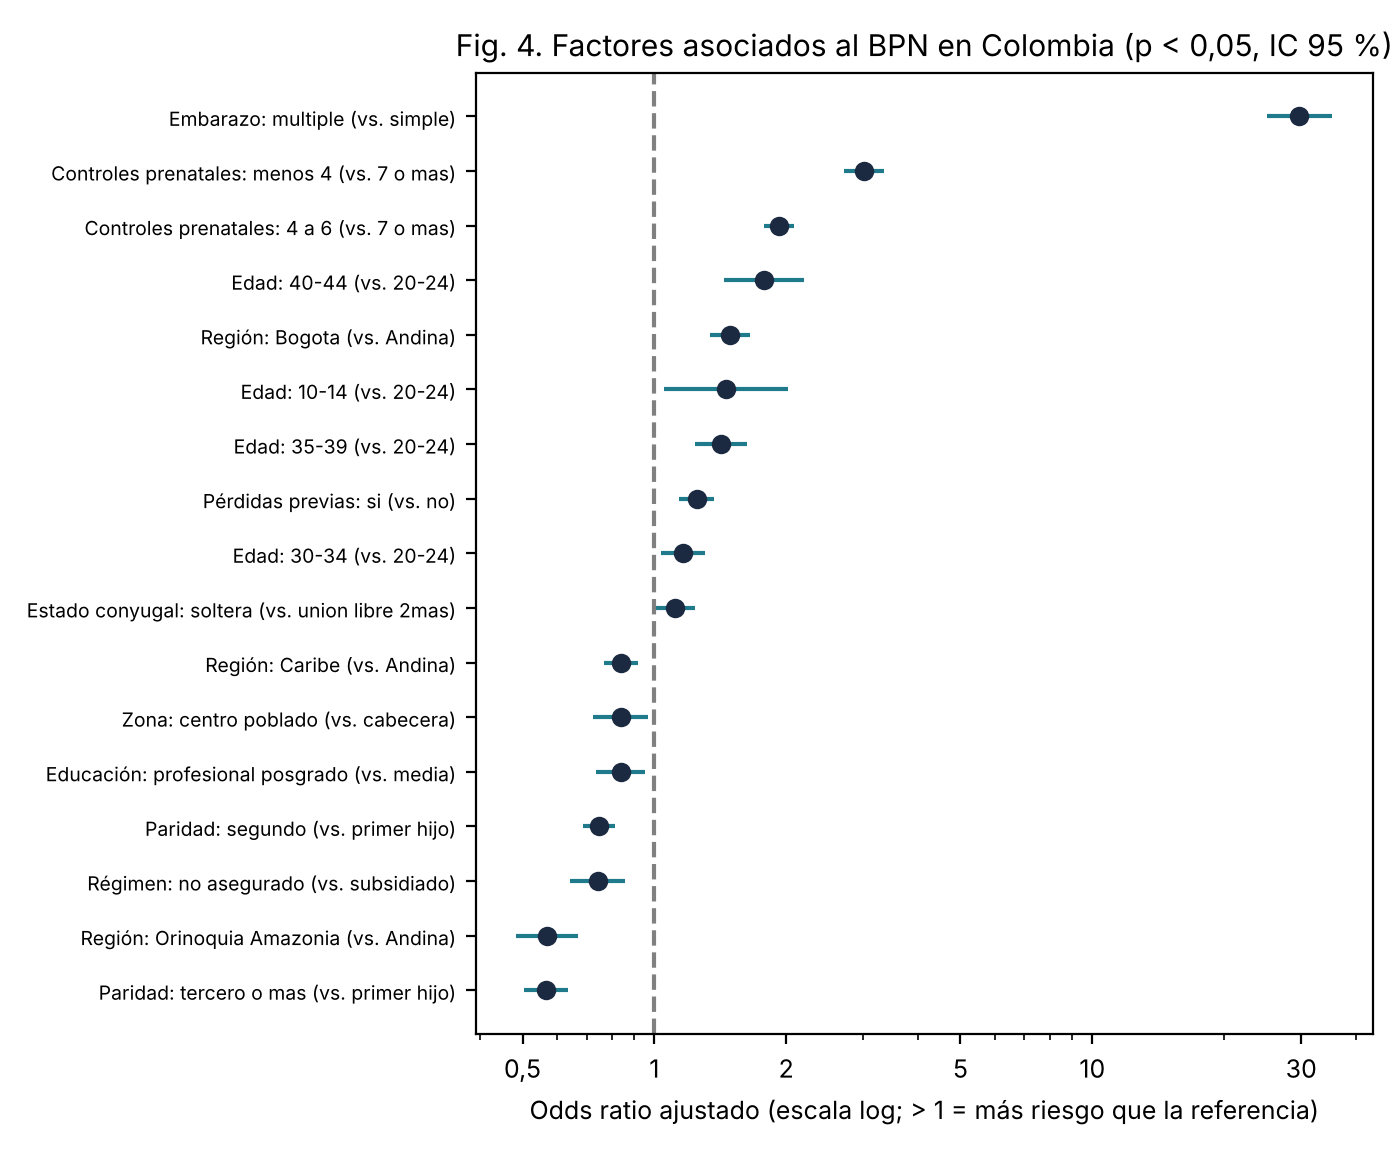
\includegraphics[width=0.78\textwidth]{fig4_odds_ratios.png}
\caption{Odds ratios ajustados (escala logarítmica). \textbf{Qué leer:} a la derecha de 1 aumentan el riesgo; el embarazo múltiple, los pocos controles y Bogotá son los factores más claros.}
\label{fig:or}
\end{figure}

\textbf{Diálogo con el artículo.} De sus cuatro factores, solo uno se puede medir con datos colombianos, y \textbf{se reproduce}: menos de cuatro controles prenatales tiene OR 3,0 (IC 2,7--3,3) en Colombia frente a 2,8 (1,1--6,8) en Etiopía, con un intervalo mucho más estrecho por el tamaño de la muestra. Consejería nutricional, perímetro braquial y estrés no se registran en el certificado de nacido vivo, así que no se pueden confirmar ni descartar. Lo que aporta el contexto local son factores que el artículo no podía ver: embarazo múltiple, altitud y edades extremas.

\textbf{Mensaje central.} \emph{Con la información que Colombia registra antes del parto se puede ordenar a las gestantes por riesgo de bajo peso al nacer ---el 20~\% de mayor riesgo concentra cerca del 40~\% de los casos--- y se confirma que menos de cuatro controles prenatales triplica las odds, como en el artículo. Pero el modelo no ve gran parte de los casos, porque las causas clínicas y nutricionales no quedan en el registro.}

% ---------------------------------------------------------------- 4
\section{Calidad, limitaciones y proyección}

\begin{itemize}
\item \textbf{Variables ausentes.} Tres de los cuatro factores del artículo no existen en los datos. El poder predictivo modesto (PR-AUC 0,27) refleja esa falta de información clínica.
\item \textbf{Controles prenatales y prematurez.} Un embarazo más corto alcanza a tener menos controles, y la prematurez es la principal vía al BPN. Sin esta variable, la PR-AUC baja de 0,273 a 0,248 pero sigue 2,4 veces por encima del azar; su OR es una asociación y no debe leerse como efecto causal.
\item \textbf{Robustez.} Con solo embarazos simples los odds ratios casi no cambian (menos de cuatro controles: 3,05; Bogotá: 1,50), así que las conclusiones no dependen del embarazo múltiple.
\item \textbf{Registro.} Los datos son administrativos: puede haber errores de digitación y diferencias de cobertura entre regiones. Se usó una muestra de 2022; los resultados no se han validado en otros años.
\item \textbf{Generalización.} La PR-AUC en prueba (0,266) cae dentro de la variación observada en validación cruzada (0,273 $\pm$ 0,012), así que no hay señales de sobreajuste: con 54 coeficientes y casi 40.000 registros el modelo tiene poco margen para memorizar. El riesgo de generalización está más en el tiempo y el lugar que en el modelo.
\item \textbf{Asociación, no causalidad.} Los odds ratios describen asociaciones ajustadas y la región es un indicador indirecto de la altitud.
\end{itemize}

\textbf{Mejoras y proyección.} (i) Enlazar con datos clínicos del control prenatal (perímetro braquial, hemoglobina, preeclampsia) para medir los factores del artículo en Colombia; (ii) usar la altitud del municipio en vez de la región; (iii) validar con otros años (2023--2024); y (iv) en \emph{Machine Learning II}, probar modelos no lineales y ensambles (árboles, bosques aleatorios, \emph{boosting}) que capten interacciones, por ejemplo entre edad, paridad y controles, comparándolos con esta logística como referencia interpretable.

\textbf{Uso de inteligencia artificial.} Se usó un asistente de IA (Claude, de Anthropic) como apoyo para programar, revisar el código y redactar. Las decisiones de modelamiento, la verificación de las cifras contra las salidas del cuaderno y la interpretación son responsabilidad del autor.

% ---------------------------------------------------------------- REFERENCIAS
\section*{Referencias}
\small
\begin{enumerate}[label={[\arabic*]},leftmargin=2em]
\item Feyisa BR, Mulatu Y, Fentahun F, Biru B, Atlantis E. Nutrition, stress, and healthcare use during pregnancy are associated with low birth weight: evidence from a case--control study in West Ethiopia. \emph{Frontiers in Public Health}. 2023;11:1213291. \url{https://doi.org/10.3389/fpubh.2023.1213291}
\item Departamento Administrativo Nacional de Estadística (DANE). Estadísticas Vitales (EEVV): nacimientos 2022. Microdatos anonimizados. Bogotá: DANE. Catálogo de microdatos, consultado en noviembre de 2026.
\item DANE. Certificado de nacido vivo (formato e instrucciones de diligenciamiento). \url{https://www.dane.gov.co/files/investigaciones/poblacion/certificados/CNacidoVivo.pdf}
\item DANE. Anuario de Estadísticas Vitales 2019: variables relacionadas con el nacido vivo. \url{https://www.dane.gov.co/files/investigaciones/poblacion/anuario-EEVV-2019/VARIABLES-RELACIONADAS-CON-EL-NACIDO-VIVO.pdf}
\item Saito T, Rehmsmeier M. The precision-recall plot is more informative than the ROC plot when evaluating binary classifiers on imbalanced datasets. \emph{PLoS ONE}. 2015;10(3):e0118432. \url{https://doi.org/10.1371/journal.pone.0118432}
\item López-Camelo JS, Campaña H, Santos R, Poletta FA. Effect of the interaction between high altitude and socioeconomic factors on birth weight in a large sample from South America. \emph{American Journal of Physical Anthropology}. 2006;129(2):305--310. \url{https://doi.org/10.1002/ajpa.20274}
\item Jensen GM, Moore LG. The effect of high altitude and other risk factors on birthweight: independent or interactive effects? \emph{American Journal of Public Health}. 1997;87(6):1003--1007. \url{https://doi.org/10.2105/ajph.87.6.1003}
\item James G, Witten D, Hastie T, Tibshirani R. \emph{An Introduction to Statistical Learning, with Applications in Python}. Springer; 2023.
\item Pedregosa F, Varoquaux G, Gramfort A, \emph{et al.} Scikit-learn: Machine Learning in Python. \emph{Journal of Machine Learning Research}. 2011;12:2825--2830.
\item Seabold S, Perktold J. Statsmodels: econometric and statistical modeling with Python. En: \emph{Proceedings of the 9th Python in Science Conference}; 2010. p.~92--96.
\end{enumerate}

\end{document}
